\section{了解计算机硬件架构}

\subsection{一般计算机硬件架构}

这里介绍一下运行操作系统的基本计算机硬件架构。一台计算机可抽象一台以图灵机(Turing Machine)为理想模型,以冯诺依曼架构( Von Neumann Architecture)为实现模型的电子设备,包括CPU、memory和 I/O 设备。CPU(中央处理器,也称处理器) 执行操作系统中的指令,完成相关计算和读写内存,物理内存保存了操作系统中的指令和需要处理的数据,外部设备用于实现操作系统的输入(键盘、硬盘),输出(显示器、并口、串口),计时(时钟)永久存储(硬盘)。操作系统除了能在计算机上运行外,还要管好计算机。下面将简要介绍计算机硬件以及操作系统大致要完成的事情。



\subsubsection{CPU} 

CPU是计算机系统的核心,目前存在各种8位,16位,32位,64位的CPU,应用在从嵌入式系统到巨型机等不同的场合中。CPU从一加电开始,从某设定好的内存地址开始,取指令,执行指令,并周而复始地运行。取指令的过程即从某寄存器(比如,程序计数器)中获取一个内存地址,从这个内存地址中读入指令,执行机器指令,不断重复,CPU运行期间会有分支和调用指令来修改程序计数器,实现地址跳转,否则程序计数器就自动加1,让CPU从下一个内存地址单元取指令,并继续执行。

由于CPU执行速度很快(x86 CPU可达到2GHZ以上的时钟频率,RISC-V CPU可达到1.5 GHZ的时钟频率),如果当前可以运行的程序太少,则会出现CPU无事可做的情况,导致计算机系统效率太低。这时就需要操作系统来帮忙了,我们需要操作系统除了能管理硬件外,还能管理应用程序,让它们能够按一定的顺序和优先级来依次使用CPU,充分发挥CPU的效能。操作系统管一个程序比较容易,但如果管理多个程序的运行,就需要考虑如何分配CPU资源的问题,如何避免程序执行期间发生“冲突”的问题等,这是操作系统需要完成的重要功能之一。

\subsubsection{memory}

计算机中有多种多层次的存放数据和指令代码的硬件存储单元,比如在CPU内的寄存器(register)、高速缓存(cache)、内存(memory)、硬盘、磁带等。寄存器位于CPU内部,其访问速度最快但成本昂贵,在对于传统的CISC(复杂指令集计算机,如Intel 80386处理器)中一般只有几个到十个左右的通用寄存器,而对于RISC(精简指令集计算机,如RISC-V),则可能有几十个以上通用寄存器;高速缓存(cache)  一般也在CPU内部,cache是内存和寄存器在速度和大小上的折衷,比寄存器慢2~10倍,容量也有限,量级大约几百KB到几十MB不等;再接下来就是内存了,内存位于CPU外,比寄存器慢10倍以上,但容量大,目前一般以几百兆B到几百GB不等;硬盘容量更大,但一般比寄存器要慢1000倍以上,不过掉电后其存储的数据不会丢失。

由于寄存器、cache、内存、硬盘在读写速度和容量上的巨大差异,所以需要操作系统来协调数据的访问,尽量主动协助应用软件,把最近访问的数据放到寄存器或cache中(实际上操作系统不能直接控制cache的读写),把经常访问的数据放在内存中,把不常用的数据放到硬盘上,这样可以达到让多个运行的应用程序“感觉”到它可用使用很大的空间,也可有很快的访问速度。如何让在运行中的每个程序都能够得到“足够大”的内存空间,且程序间相互不能破坏对方的内存“领地”,且建立他们之间的“数据共享”通道,这是操作系统需要完成的重要功能之一。

\subsubsection{I/O}


CPU处理的数据需要有来源和输出,这里的来源和输出就是各种外设,如大家日常使用计算机用到的键盘、鼠标、显示器、声卡、GPU、U盘、硬盘、SSD存储、打印机、网卡、摄像头等。上图中给出了PC计算机的一些外设硬件。应用程序如果直接访问外设,会有代码实现复杂,可移植性差,无法有效并发等问题,所以操作系统给应用程序提供了简单的访问接口,让应用程序不需要了解硬件细节。具体访问外设的苦活累活都交给操作系统来完成了,这就是操作系统中外设驱动哦程序的主要功能。

如果操作系统要通过CPU对数据进行加工,首先需要有输入,在处理完后还要进行输出,否则没东西要处理或者执行完了无法把结果反馈给用户。操作系统要处理的数据需要从外设(比如键盘、串口、硬盘、网卡)中获得,这就是一种读外设数据的操作;且在处理完毕后要传给外设(比如显示器、硬盘、打印机、网卡)进一步处理,这其实就是一种写外设数据的操作。

一般而言,IO外设把它的访问接口映射为一块内存区域,操作系统通过来用通常的内存读写指令来管理设备;或者CPU提供了特定的IO操作指令,操作系统通过这些特定的指令来完成对IO外设的访问。并且操作系统可以通过轮循、中断、DMA等访问方式来高效地管理外设。

比如,在RISC-V中通过对特定地址的内存(代表IO外设的接口)进行读或写访问,就可以实现对IO外设的访问了。在Intel x86中有两条特殊的 in和out 指令来在完成CPU对外设地址空间的访问,实现对外设的管理控制。本书不会涉及很多复杂具体硬件,而只涉及到操作系统用到的一些最基本的外设硬件(时钟,串口,硬盘)细节。


\subsection{RISC-V硬件架构}\label{riscv}

通用CPU一般能够在硬件上支持内存空间的隔离,使得多个程序在各自独立的内存空间中并发执行。这种硬件机制即支持用户特权级和内核特权级。应用程序运行在用户特权级,这样应用不能执行特权指令,且不能破坏操作系统内核的数据和操作系统执行过程。而操作系统内核运行在内核特权级,可以访问特权指令,并管理和控制应用程序,硬件外设等。所以对于操作系统而言,需要CPU硬件至少支持用户特权级和内核特权级(控制隔离),以及内存空间隔离(数据隔离)。

RISC-V是发源于Berkeley的开源instruction set architecture
(ISA)。在继续阅读前,对RISCV指令集和架构特别感兴趣的同学可仔细阅读RISC-V的Specifications。当前用户态指令集规范的版本为2.2,特权态指令集规范的版本为1.10。

\begin{itemize}
\item
  \href{https://riscv.org/specifications/}{User-Level ISA Specification
  v2.2}
\item
  \href{https://riscv.org/specifications/privileged-isa}{Draft
  Privileged ISA Specification v1.10}
\end{itemize}

\subsection{Modular ISA}\label{modular-isa}

RISC-V ISA是模块化的,它由一个基本指令集和一些扩展指令集组成

\begin{itemize}
\item
  Base integer ISAs

  \begin{itemize}
  \item
    RV32I
  \item
    RV64I
  \item
    RV128I
  \end{itemize}
\item
  Standard extensions

  \begin{itemize}
  \item
    M: Integer \textbf{M}ultiply
  \item
    A: \textbf{A}tomic Memory Operations
  \item
    F: Single-percison \textbf{F}loating-point
  \item
    D: \textbf{D}ouble-precision Floating-point
  \item
    G: IMAFD, \textbf{G}eneral Purpose ISA
  \end{itemize}
\end{itemize}

举例来说,\texttt{RV32IMA}表示支持基本整数操作和原子操作的32位RISC-V指令集。对于一般在用户态执行的应用程序,只需要上述用户态指令集就基本足够了。但如果是象操作系统这样的软件,需要控制整个计算机硬件,则只使用用户态指令集是不够的,还需要在处于内核特权级的CPU状态下执行特权指令集。

\subsection{Privileged ISA}\label{privileged-isa}

\subsubsection{Software Stacks}\label{software-stacks}

RISC-V在设计时就考虑了硬件虚拟化的需求,三种典型RISC-V系统的结构如下

%\begin{figure}[htbp]
%\centering
%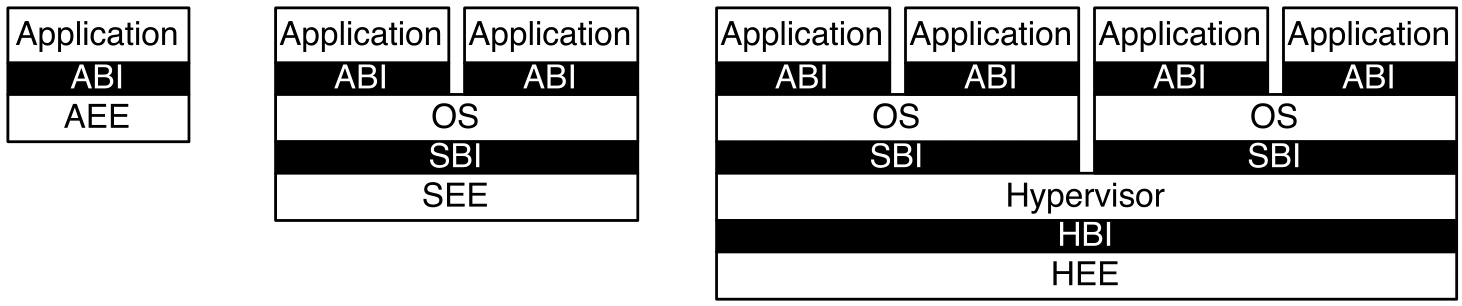
\includegraphics{figures/software-stacks.png}
%\caption{software-stacks}
%\end{figure}

上图中各个英文缩写对应的全称如下

\begin{itemize}
\item
  ABI: Application Binary Interface
\item
  AEE: Application Execution Environment
\item
  SBI: Supervisor Binary Interface
\item
  SEE: Supervisor Execution Environment
\item
  HBI: Hypervisor Binary Interface
\item
  HEE: Hypervisor Execution Environment
\end{itemize}

RISC-V通过各层之间的Binary
Interface实现了对下一层的抽象,方便了虚拟机的实现以及OS在不同RISC-V架构间的移植。采用了图中第二种结构,\href{https://github.com/riscv/riscv-pk}{bbl}在其中充当了SEE的角色。

\subsubsection{Privilege Levels}\label{privilege-levels}

RISC-V共有4种不同的特权级,与x86不同的是,RISC-V中特权级对应数字越小,权限越低

\begin{longtable}[c]{@{}cccc@{}}
\toprule
Level & Encoding & Name & Abbreviation\tabularnewline
\midrule
\endhead
0 & 00 & User/Application & U\tabularnewline
1 & 01 & Supervisor & S\tabularnewline
2 & 10 & Hypervisor & H\tabularnewline
3 & 11 & Machine & M\tabularnewline
\bottomrule
\end{longtable}

一个RISC-V的实现并不要求同时支持这四种特权级,可接受的特权级组合如下

\begin{longtable}[c]{@{}cll@{}}
\toprule
Number of levels & Supported Modes & Intended Usage\tabularnewline
\midrule
\endhead
1 & M & Simple embedded systems\tabularnewline
2 & M, U & Secure embedded systems\tabularnewline
3 & M, S, U & Systems running Unix-like operating systems\tabularnewline
4 & M, H, S, U & Systems running Type-1 hypervisors\tabularnewline
\bottomrule
\end{longtable}

目前官方的\href{https://github.com/riscv/riscv-isa-sim}{Spike}模拟器只部分实现了3个特权级。

\subsubsection{Control and Status
Registers}\label{control-and-status-registers}

RISC-V中各个特权级都有单独的Control and Status Registers
(CSRs),其中应当注意的有以下几个

\begin{longtable}[c]{@{}ll@{}}
\toprule
Name & Description\tabularnewline
\midrule
\endhead
sstatus & Supervisor status register\tabularnewline
sie & Supervisor interrupt-enable register\tabularnewline
stvec & Supervisor trap handler base address\tabularnewline
sscratch & Scratch register for supervisor trap handlers\tabularnewline
sepc & Supervisor exception program counter\tabularnewline
scause & Supervisor trap cause\tabularnewline
sbadaddr & Supervisor bad address\tabularnewline
sip & Supervisor interrupt pending\tabularnewline
sptbr & Page-table base register\tabularnewline
mstatus & Machine status register\tabularnewline
medeleg & Machine exception delegation register\tabularnewline
mideleg & Machine interrupt delegation register\tabularnewline
mie & Machine interrupt-enable register\tabularnewline
mtvec & Machine trap-handler base address\tabularnewline
mscratch & Scratch register for machine trap handlers\tabularnewline
mepc & Machine exception program counter\tabularnewline
mcause & Machine trap cause\tabularnewline
mbadaddr & Machine bad address\tabularnewline
mip & Machine interrupt pending\tabularnewline
\bottomrule
\end{longtable}

在继续阅读前,读者应当查阅\href{https://riscv.org/specifications/privileged-isa}{Privileged
Spec 1.9.1}以熟悉以上CSR的功能和用途。

\paragraph{CSR Instructions}\label{csr-instructions}

RISC-V
ISA中提供了一些修改CSR的原子操作,下面介绍之后常用到的\texttt{csrrw}指令

\begin{lstlisting}[language={C}]
# Atomic Read & Write Bit
cssrw rd, csr, rs
\end{lstlisting}

语义上等价的C++函数如下

\begin{lstlisting}[language={C}]
void cssrw(unsigned int& rd, unsigned int& csr, unsigned int& rs) {
   unsigned int tmp = rs;
   rd = csr;
   csr = tmp;
}
\end{lstlisting}

几种有趣的用法如下

\begin{lstlisting}[language={C}]
# csr = rs
cssrw x0, csr, rs

# csr = 0
cssrw x0, csr, x0

# rd = csr, csr = 0
cssrw rd, csr, x0

# swap rd and csr
cssrw rd, csr, rd
\end{lstlisting}

